%!TEX root = ../main.tex

\chapter{Einleitung}
Diese Dokumentation soll einen Einblick in die Architektur der


\chapter{Kafka}
Um Nachrichten zwischen verschiedenen Komponenten in Echtzeit auszutauschen wird in größeren Systemen Kafka verwendet. Kafka ist eine Event Streaming Plattform die von der Apache Software Foundation bereitgestellt wird. Sie ist eine Open-Source Software. Eingesetzt wird Kafka in Bereichen in denen eine Komponente Daten auswirft und eine andere Komponente diese Daten sofort verarbeiten soll, dieses Szenario tritt in Banksystemen auf wo eine Geldtransaktion so schnell wie möglich verarbeitet werden soll. Wichtig hierbei ist auch die Sicherheit, selbstverständlich sollten keine Transaktionen verloren gehen. Um dies zu vermeiden ist Kafka in der Lage die gesendeten Daten für eine unbegrenzte Zeit zuverlässig zu speichern. Ein anderer Einsatzort von Kafka ist im Internet of Things Bereich, hier werden Sensordaten von den verschiedenen IoT Geräten an Kafka übertragen und von dort kann dann eine Komponente diese Daten auslesen und verarbeiten. Die Skalierbarkeit von Kafka ist ein großer Vorteil. Es können viele produzierende und verarbeitende Komponenten mit Kafka verwendet werden, im IoT Bereich werden viele Geräte Daten senden und diese können dann von wenigen Komponenten verarbeitet werden. Um mit beiden Seiten mit zu skalieren werden sogenannte Cluster in Kafka gebildet. Ein Cluster besteht aus einem oder mehr Kafka Instanzen diese arbeiten zusammen um die Daten zu empfangen, speichern und zu versenden. Für eine erhöhte Ausfallsicherheit und um die Last zu verteilen werden normalerweise immer mindestens drei Kafka Instanzen zusammen verwendet. Dieses Cluster kann falls eine Kafka Instanz ausfällt dies ausgleichen und die Arbeit auf die laufenden Kafka Instanzen verteilen, hierbei gehen auch keine Daten verloren. Die Daten in den Kafka Instanzen, die auch Broker genannt werden, werden repliziert, dass bedeutet mehrere Broker besitzen die gleichen Daten. Dadurch gehen keine Daten verloren selbst wenn ein oder mehr Broker ausfallen. Wenn etwas in dem System passiert, dazu zählen Sensordaten Ermittlung und anstoßen einer Transaktion, wird dies als Event in Kafka festgehalten. Diese Events können auch Nachricht genannt werden, da diese auch zur Übertragung dienen. Ein Producer in Kafka ist eine Anwendung die Events/Nachrichten in das Kafka Cluster schreibt. Die andere Seite wird Consumer genannt, diese Anwendungen lesen die Daten aus dem Kafka Cluster und verarbeiten sie. Durch diese Trennung der Einheiten ist Kafka viel skalierbarer, alle drei Einheiten können unabhängig voneinander skaliert werden. Für gewöhnlich wird das Cluster in der Skalierung an die Consumer und Producer angepasst, da über dieses alle Events durchgehen und es somit mit beiden Seiten mithalten muss. Wenn ein Event in das Cluster eingeht wird es in einem Topic gespeichert, ein Topic ist von der Arbeitsweise ähnlich zu einem normalen Dateiverzeichnis. Alle Topics in Kafka können null, ein oder viele Producer haben und auch null, ein oder viele Consumer haben. Ein unterschied den Topics zu anderen Nachrichtensystemen haben ist das die Events die gespeichert sind nicht nach dem lesen entfernt werden. Ein Event kann so oft wie nötig gelesen werden, dieses Verhalten kann für jedes Topic eingestellt werden. Ebenfalls lässt sich einstellen wie lange die Events gespeichert bleiben sollen bevor sie gelöscht werden.

\begin{figure}[H]
	\centering
	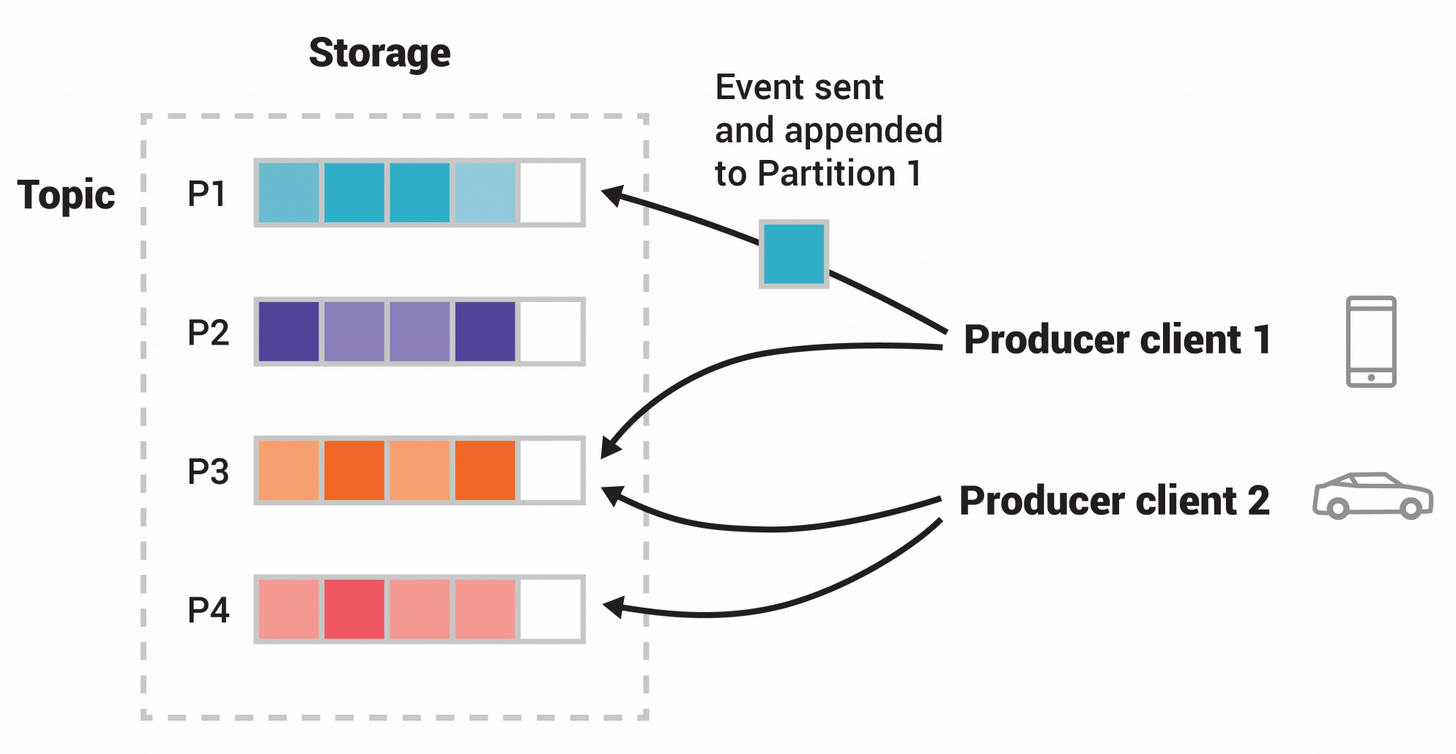
\includegraphics[width=1\linewidth]{resources/images/partition}
	\caption{Hier ist die Partitionierung mit zwei Producern dargestellt.}
	\label{fig:Partition}
\end{figure}

Die Topics sind partitioniert, das bedeutet das Teile des Topics auf verschiedenen Kafka Brokern liegt. Diese Verteilung verbessert die Skalierbarkeit, da in mehreren Brokern gleichzeitig gelesen und geschrieben werden kann. Wie bereits angesprochen können Daten repliziert werden, genauer werden die Topics auf verschiedene Broker repliziert.